% This is samplepaper.tex, a sample chapter demonstrating the
% LLNCS macro package for Springer Computer Science proceedings;
% Version 2.20 of 2017/10/04
%
\documentclass[runningheads]{llncs}
\usepackage[a4paper, margin=1.7cm]{geometry}
\usepackage{graphicx}
\usepackage{hyperref}
\hypersetup{colorlinks=true,
            linkcolor=black,
            citecolor=black,
            urlcolor=blue}

% Used for displaying a sample figure. If possible, figure files should
% be included in EPS format.
%
% If you use the hyperref package, please uncomment the following line
% to display URLs in blue roman font according to Springer's eBook style:
% \renewcommand\UrlFont{\color{blue}\rmfamily}


\begin{document}

%

\begin{titlepage} % Suppresses displaying the page number on the title page and the subsequent page counts as page 1
	\newcommand{\HRule}{\rule{\linewidth}{0.5mm}} % Defines a new command for horizontal lines, change thickness here
	
	\center % Centre everything on the page
	
	%------------------------------------------------
	%	Headings
	%------------------------------------------------
	\vspace{5em}
	\textsc{\LARGE Université de Rennes 1}\\[1.5cm] % Main heading such as the name of your university/college
	
	\vspace{3em}
	\textsc{\Large\bfseries EDD}\\[0.5cm] % Major heading such as course name
	\textsc{\large Data Warehouses}\\[0.5cm] % Minor heading such as course title
	
	%------------------------------------------------
	%	Title
	%------------------------------------------------
	
	\vspace{5em}
	\HRule\\[0.4cm]
	
	{\huge\bfseries Open Food Facts Project}\\[0.4cm] % Title of your document
	
	\HRule\\[1.5cm]
	
	%------------------------------------------------
	%	Author(s)
	%------------------------------------------------
	
	\vspace{5em}
	\begin{minipage}{0.4\textwidth}
		\begin{flushleft}
			\large
			\textit{Authors}\\
			\textsc{D. De Paola}\\
			\textsc{L. Mandruzzato}
			 % Your name
		\end{flushleft}
	\end{minipage}
	~
	\begin{minipage}{0.4\textwidth}
		\begin{flushright}
			\large
			\textit{Supervisor}\\
			 \textsc{Prof. Marc Bousse} % Supervisor's name
		\end{flushright}
	\end{minipage}
	
	% If you don't want a supervisor, uncomment the two lines below and comment the code above
	%{\large\textit{Author}}\\
	%John \textsc{Smith} % Your name
	%\thispagestyle{plain}
	\vspace{10em}
	\begin{abstract}
	    This paper describes the design process of a multidimensional model for analyzing data coming from the Open Food Facts platform. It aims to find an efficient solution to support Online Analytical Processes (OLAP). We can divide the followed approach into three main steps. Firstly, a design phase (sections \ref{design} and \ref{ER}) — i.e., UML modeling \cite{UML} and ER schema design \cite{ER}. Secondly, an implementation stage (sections \ref{ER} and \ref{kettle}) — i.e., SQL code to physically implement the ER schema \cite{SQL} and Kettle transformations to populate it \cite{Kettle_dim}\cite{Kettle_fact}. Finally, a querying process followed by some analysis (sections \ref{queries} and \ref{results}) — i.e., MDX queries design \cite{MDX} and discussion of the results obtained.
	    \keywords{Business Intelligence \and Kettle \and MDX \and Mondrian \and Multidimensional Models \and Pentaho \and R-OLAP}
	\end{abstract}
	
	
	%------------------------------------------------
	%	Date
	%------------------------------------------------
	
	\vfill\vfill\vfill % Position the date 3/4 down the remaining page
	
	{\large October 2021} % Date, change the \today to a set date if you want to be precise
	
	%------------------------------------------------
	%	Logo
	%------------------------------------------------
	
	%\vfill\vfill
	%\includegraphics[width=0.2\textwidth]{placeholder.jpg}\\[1cm] % Include a department/university logo - this will require the graphicx package
	 
	%----------------------------------------------------------------------------------------
	
	\vfill % Push the date up 1/4 of the remaining page
	
\end{titlepage}
\newpage
\section{Design choices for the Mondrian Schema}\label{design}

\subsection{Assignment and research directions}\label{directions}
The Open Food Facts integration base structures the data about several products in three tables. One contains the users’ pseudo, the second is reserved for the product categories — i.e., pnns1 and pnns2 — and the last with the different details for each single product update.

Leveraging data that has been given to us and the two MDX queries present in the assignment, we derived three main research directions.

\begin{enumerate}
  \item The former research scope was to retrieve the distribution of products on the platform. In this way, we can make a fast analysis of the product coverage on several categories.
  \item The second direction for information extraction was to find the update frequency for every single product, highlighting the possible presence of specific non-updated elements in the dataset and the most active typologies of contributors.
  \item A third interesting research direction has been adopted to explore the nutritional grading on different categories of products. Through it, it is possible to discover healthier clusters of products and suggest to the industry a need for nutritional quality improvement in the related area.
\end{enumerate}

\subsection{Measures}
To support the two queries given in the assignment, the following measures have been derived:

\begin{itemize}
    \item \textbf{Number of products:} the number of different products, identified by their barcode.
    \item \textbf{Number of versions:} the number of different versions, identified by their barcode and last modified field — i.e., a value derived by the date modification field.
\end{itemize}

Three additional measures have been defined to support the research directions outlined in section \ref{directions}, specifically for retrieving some useful information on the nutrition score and the number of updates:

\begin{itemize}
    \item \textbf{Average Score:} Average grade of nutrition scores.
    \item \textbf{Number of creations:} The number of new products added to the platform. It is defined by counting the number of different barcodes.
    \item \textbf{Number of updates:} Count of different updates. Defined as $Number \ of \ versions - Number \ of \ creations$
\end{itemize}

\subsection{Dimensions}\label{dim}
By following the inspection objectives defined in section \ref{directions}, the following dimensions were used to support our measures:

\begin{itemize}
  \item \textbf{Dimension Date Creation and Modification} contains a single hierarchy with the version day, month, and year of creation or modification. The dimension scheme will contain all distinct and non-duplicated dates present in the database.
  \item \textbf{Dimension Category} contains a single hierarchy defined by four levels: version, product, PNNS2, PNNS1. The dimension scheme will contain all the information related to the product, its general category, and version.
  \item\textbf{Dimension Nutritional Info (Degraded)} contains a single hierarchy defined by four levels: version, score, class, presence. The levels respectively describe the version of the nutritional score, the nutrition score associated with a product and a version, the nutrition score class — i.e., A, B, C, D, E — and the presence of the nutrition score in the integration base.
  \item\textbf{Dimension Contributors (Degraded)} contains a single hierarchy defined by two levels: contributor and type. The table contains the information about contributors and their typology — i.e., corporate or individual.
\end{itemize}

The dimension usage mapping for the different measures resulted in the table presented in figure~\ref{fig1}. From the scheme, it is possible to identify the distinction between two different cubes: the items cube (blue) and the versions cube (orange). 

\begin{figure}
    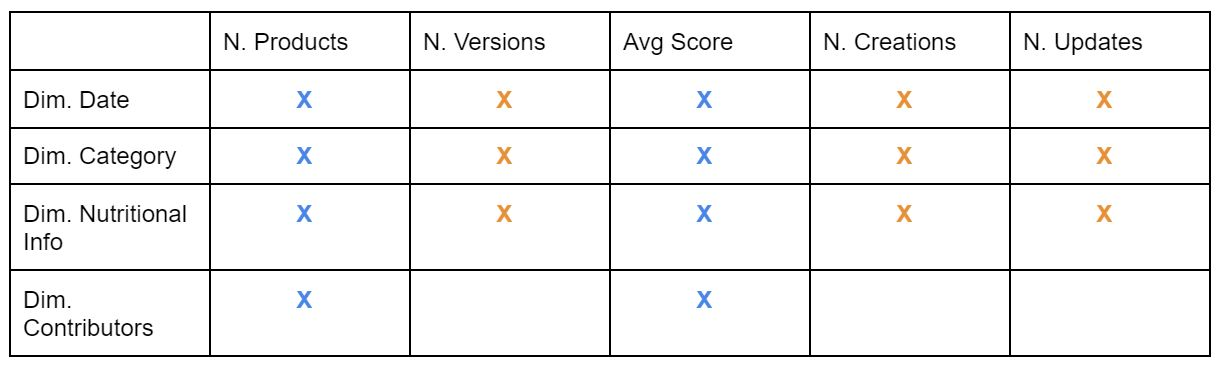
\includegraphics[width=\textwidth]{MeasuresAndDimTable.JPG}
    \caption{\emph{Mapping of Dimension usage on Measures}}
    \label{fig1}
\end{figure}

\subsubsection{Comments} Some important comments should be made on the contributors' dimension. Using the official database documentation \cite{OFF_doc} and by using some SQL test queries, it was possible to understand that, for each tuple in the versions table, only the original creator pseudo is provided. Since the contributor field does not change between different versions of a single product, it makes no sense to add this dimension in a cube that keeps into account the versions. Not only it is meaningless, but it can also bias the analysis. For instance, considering a brand new user A that adds a new product to the DB, and the latter is updated 20 times by other profiles, it would appear that user A is very active even though he has only created one single product. For this reason, as we will explain in section \ref{cubes}, we designed a cube that contains only the last updated versions for each barcode. In this way, it would appear that contributor A has interacted with the platform only once, which is correct.

\subsection{Cubes}\label{cubes}
\begin{description}
    \item[Items Cube] The Items cube contains all the information required to support the analysis on the homogeneous updated distribution of products and the different average nutrition score on different items categories, following the first and third inspection objective defined in section \ref{directions}. 
    \item[Version Cube] The Versions cube will instead support the analysis on the frequency of updates and the identity of the most important contributors for different categories — i.e., the second direction of section \ref{directions}.
\end{description}

In the final XML, the nutritional value presence (present or NULL), the nutritional category (A, B, C, D, E), and the contributor typology (corporate or individual) have been managed through key expressions.
 
\section{Relational Model}\label{ER}
The relational schema adopted for our Data Mart is made of two dimensional tables and two facts tables: OFF\_dim\_date, OFF\_dim\_category, OFF\_items\_facts, and OFF\_versions\_facts. 
As clarified in section \ref{dim}, the dimensions Nutritional Score and Contributors have been degraded into the fact tables. A nutr\_score column was added to both the fact tables, while the pseudo field (contributors' identifier) was only included in the items fact table. 

Different choices were made in the process of populating the database.

As concerns the two dimension tables, we can notice a slight difference between them. While for the category we used both a business key — i.e., version — and a technical key — i.e., TECH\_KEY\_CAT, for the date we only exploited the technical one — i.e., TECH\_KEY\_DATE. The introduction of the two technical keys, as in many examples seen during the lectures, simplified the populating processes and was extremely useful in the Kettle pipelines (section \ref{kettle}) used for loading the data.

As already anticipated in section \ref{cubes}, being the items cube used for the study of the actual distribution of products into the platform, the items fact table was populated with the foreign keys of the last updated versions — i.e., we want to have the last/current state of the product. The versions cube, instead, was populated by importing all the versions present into the integration base, referenced with their correspondent technical keys. 

\section{Kettle}\label{kettle}

We exploited an ETL tool delivered by Pentaho named Data Integration (Kettle) to populate the Data Mart. Through it, we managed to extract the necessary data from the integration base, transform it, and finally load it into the warehouse.
We designed two different transformations, one for the dimension tables and the other for the fact tables. To be run, both of them need that the SQL script to create the structure of the DB — i.e., tables and fields — was already executed.

\subsection{Dimension Tables Transformation}
We know that there are two dimension tables to be populated (see section physical model). Both of them will have a correspondent pipeline within the transformation — i.e., a process that takes care to fill it. Inside each table, we can distinguish a certain number of fields and a technical primary key — i.e., a sequential number assigned from the database. It is necessary to have the latter before executing the second transformation because it represents the fact table foreign key. Thus, we can notice a specific execution order: complete the dimension tables before filling the fact ones.
We can observe a structure shared by the pipelines. Firstly, a sub-part to retrieve data from the integration base. Since we prefer to query the BI as few times as possible, we used a single component to accomplish this task for all four pipelines. After the retrieving process, for the date dimension, there is a component dedicated to filtering duplicates because we do not want different rows containing the same date. This process is fundamental for the next transformation to execute the DB lookup component to retrieve the sequential keys to add in the fact tables. In fact, after having removed duplicates, each row of the date dimension can be individuated using the primary key, but even using the set of all the other data — i.e., day, month, year. In the end, there are some steps focused on populating the already existing dimension tables with the data obtained from the stream.
\subsection{Fact Tables Transformation}
Even here, there is a structure shared between the two pipelines which populate the OFF\_items\_facts and OFF\_versions\_facts. It consists of an initial retrieving/creating sub-part that collects and adds all the fields necessary to obtain the technical keys. Thus, at the end of this process, we must have a stream containing all the data that distinguish all the sequential keys to fill each fact table. In a nutshell, if in a dimension table there is a row with “1” as technical sequential key and “A” and “B” as other data, that instance can be retrieved passing to the query “1” as a parameter, but even using “A” and “B”. The latter querying typology is the one executed from the DB lookup component present after the first sub-part of the transformation. There is one of them for both the dimensions considered for each fact table. In the end, after having obtained the sequential keys — i.e., the foreign keys, we can proceed to put the results in the tables.


\section{MDX Queries}\label{queries}
The MDX queries design process can be ideally split into two different moments. One during the first step of the project in order to frame the problem and get an idea of the measures and dimensions we would have needed. We can see these initial queries as guidelines to follow to have more clear the problem to solve. At a later time, after having a functioning version of our multidimensional model, we focused again on MDX queries to improve them. After having worked on the model, we were more aware of its potential and of what could and could not be done with it.

\subsection{Query Description}
\subsubsection{Items Cube}
\begin{itemize}\label{itemsQueries}
  \item \textbf{Query n.1.} This query computes the number of product descriptions per creator and year of creation on rows (assigned query).
  \item \textbf{Query n.2.} This query verifies that the items cube works properly. If everything is correct, this query should return no results, because there are no barcodes that appear twice in the table (no versions, only products).
  \item \textbf{Query n.3.} This query spots which are the most and less healthy PNNS2 categories.
  \item \textbf{Query n.4.} This query highlights the categories that have a lack of information related to the nutritional score.
  \item \textbf{Query n.5.} This query gets information about how the different typologies of contributors impact the system adding products. Which are the "most active" categories of contributors?
  \item \textbf{Query n.6.} This query retrieve the number of products for the different pnns1 and pnns2 on columns per years on rows. 
\end{itemize}
\subsubsection{Versions Cube}\label{versionsQueries}
\begin{itemize}
    \item \textbf{Query n.1.} This query computes the number of versions per month on rows and PNNS1 values on columns of all product descriptions created in 2017 (assigned query). We can have updates even later than 2017, the only constraint is that the creation date of the products in question is dated in that year.
    \item \textbf{Query n.2.} This query allows understanding the number of updates per each product creation for each category.
    
\end{itemize}

\section{Results}\label{results}
The MDX queries defined in the previous section support the three research directions set at the beginning: the coverage of products on different categories, the frequency of updates performed on the products, and the average nutritional score for several classes. 

For the first analysis scope, we considered the results of queries number 1, 5, and 6 on the items cube (section \ref{itemsQueries}). By the resulting aggregate table retrieved on Pentaho, it is possible to verify the general distribution of products on the platform. Regarding the contributors, we can spot that the proportion of individual contributions is higher than the corporate one in almost every product category. We can expect it for a crowdsourcing platform as Open Food Facts. Moreover, it is a perfect parameter to test the heterogeneous distribution of contributors. Examining the results of the first query, we can also monitor the number of corporate contributions on the platform and discover a high activity in 2016 and a declining trend for the following years. A new strategy to engage Corporate Companies could be suggested to the Open Food Facts project.

Regarding the frequency of updates, we took into examination the results on queries number 1 and 2 on the version cube (section \ref{versionsQueries}). From the first query, it is possible to understand the number of different versions for the products created in 2017. The results for the second query allow monitoring the rate between creations and updates for each PNNS1 category. On average, the rate of updates is very high, meaning that each of the PNNS1 categories is frequently updated. 

Finally, to retrieve some insights on the nutritional score, we studied the result deriving from queries 3 and 4 on the Items Cube (section \ref{itemsQueries}). From the first query, it was possible to verify which categories have more 'null' nutritional scores. From the second one, it is possible to find the classes with lower average nutrition score. For the category "Non-sugared beverages" could be advisable to reduce the number of 'null' nutritional scores. A final and extremely interesting result regards the average nutrition scores. The low average on some common categories such as “breakfast cereals” and ”dressing and sauces”, could be a piece of extremely valuable information for a company, suggesting the creation of new healthier products for that category. In a nutshell, this analysis may suggest to a company a possible blue ocean \cite{Blue_ocean} in which enter with brand new products.


\begin{thebibliography}{8}

\bibitem{UML}
UML Cubes - \href{https://drive.google.com/file/d/1OXqoUHYORNAeoYiIW48qWie1biFImclk/view?usp=sharing}{OFF\_UML\_cubes.pdf}

\bibitem{ER}
ER Schema - \href{https://drive.google.com/file/d/1Tj3Ff4SW5SalN-cHz-3SFPpiQvsAFUIA/view?usp=sharing}{OFF\_ER\_schema.pdf}

\bibitem{Mondrian}
Mondiran XML schema - \href{https://drive.google.com/file/d/1lJUrINv4cD8bpt_rbguRNqbTZdhZK1_4/view?usp=sharing}{OFF\_mondrian\_schema.xml}

\bibitem{SQL}
SQL script to create physical DB - \href{https://drive.google.com/file/d/1eCghbQvV1YWos_ByLT7d3WKadAA7giW8/view?usp=sharing}{OFF\_SQL\_starModel.xml}

\bibitem{Kettle_dim}
Kettle transformation for dimension tables - \href{https://drive.google.com/file/d/1stRD6mkiLHVMmi2wZulkbTej-Y6_Wq3c/view?usp=sharing}{OFF\_kettle\_dim\_tables.ktr}

\bibitem{Kettle_fact}
Kettle transformation for fact tables - \href{https://drive.google.com/file/d/1s3R28N6qIgJcUsU-3oShPSO7XPx0O5RP/view?usp=sharing}{OFF\_kettle\_fact\_tables.ktr}

\bibitem{MDX}
MDX Queries - \href{https://drive.google.com/file/d/1e_XURkhomOWtEVxNgomQYiRQHYzmzRSi/view?usp=sharing}{OFF\_MDX\_queries.txt}

\bibitem{OFF_doc}
OFF official documentation describing the fields present in their DB - \href{https://static.openfoodfacts.org/data/data-fields.txt}{data-fields.txt}

\bibitem{Blue_ocean}
Blue Ocean Strategy - \url{https://www.blueoceanstrategy.com/what-is-blue-ocean-strategy/}

\end{thebibliography}

%
% the environments 'definition', 'lemma', 'proposition', 'corollary',
% 'remark', and 'example' are defined in the LLNCS documentclass as well.
%
%

\end{document}
